%%%%%%%%%%%%%%%%%%%%%%%%%%%%%%%%%%%%%%%%%

% This template has been downloaded from:
% http://www.LaTeXTemplates.com
%
%%%%%%%%%%%%%%%%%%%%%%%%%%%%%%%%%%%%%%%%%


\documentclass{beamer}

\mode<presentation> {

\usetheme{Warsaw}


%\setbeamertemplate{footline} % To remove the footer line in all slides uncomment this line
%\setbeamertemplate{footline}[page number] % To replace the footer line in all slides with a simple slide count uncomment this line
\setbeamertemplate{navigation symbols}{} % To remove the navigation symbols from the bottom of all slides uncomment this line
}
\usepackage{amsmath}
\usepackage{graphicx} % Allows including images
\usepackage{booktabs} % Allows the use of \toprule, \midrule and \bottomrule in tables
\usepackage{mathtools}
\usepackage{bbm}
\usepackage{subcaption} %Multiple figures, 1 caption

%%TITLE PAGE
\title[Numerical methods for SDE's]{Strong Schemes for the Numerical Solution of Stochastic Differential Equations (SDE's) } % The short title appears at the bottom of every slide, the full title is only on the title page

\author{Amr Umeri} 
\institute[University of Bern] % Your institution as it will appear on the bottom of every slide, may be shorthand to save space
{
University of Bern \\ % Your institution for the title page
\medskip
\textit{amr.umeri@outlook.com} % Your email address
}
\date{\today} % Date, can be changed to a custom date

\begin{document}

\begin{frame}
\titlepage % Print the title page as the first slide
\end{frame}

\begin{frame}
\frametitle{Overview} % Table of contents slide, comment this block out to remove it
\tableofcontents % Throughout your presentation, if you choose to use \section{} and \subsection{} commands, these will automatically be printed on this slide as an overview of your presentation
\end{frame}

\section{Introduction} 

\begin{frame}
\frametitle{Introduction}
SDE = Differential equation + Noise term (Randomness)\\
Simbolycal:
\[\mathrm{d}X_t = a(X_t)\mathrm{d}t + b(X_t)\mathrm{d}W_t.\]

integral form:
\[X_t = x_0 + \int_0^t \!a(X_s)\,\mathrm{d}s + \underbrace{\int_0^t \!b(X_s)\,\mathrm{d}W_{s}}_{\text{Stochastic integral}},\quad t\in [0,T]\]
\[X_0 = x_0\,\,\text{initial value}\]
\end{frame}




\begin{frame}
\frametitle{Introduction}
\textbf{Questions:}
\begin{enumerate}
\item How to give a mathematical interpretation? 
\item What are solutions of such equations?\\ 
Existence, uniqueness? Probability distribution?
\item How to solve such equations analytically?
\end{enumerate}
\end{frame}

\begin{frame}
\frametitle{Introduction}
Solutions of stochastic differential equations are \textbf{stochastic processes}  (if it exists).\\
Figure: one \textbf{realization} of a stochastic process.
\begin{figure}
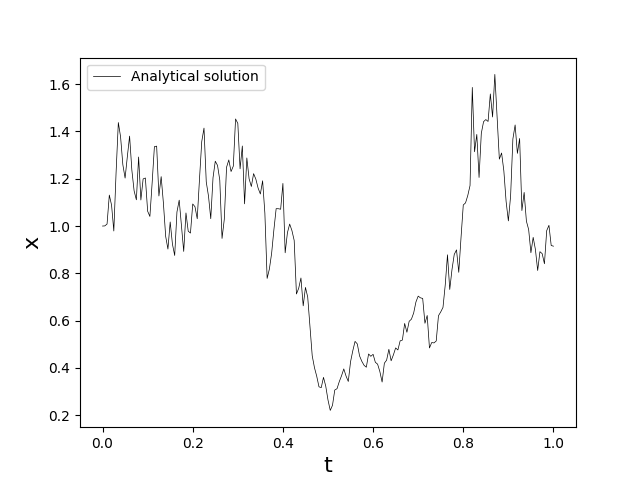
\includegraphics[width=0.6\linewidth]{Content/Graphics/slides/AnalyticalSolution}
\end{figure}
\end{frame}


\begin{frame}
\frametitle{Main goal: Construction of numerical methods for SDE's}
We want to construct numerical methods for the strong approximation of SDE's.\\
Strong: \textbf{pathwise approximation}.
\begin{figure}
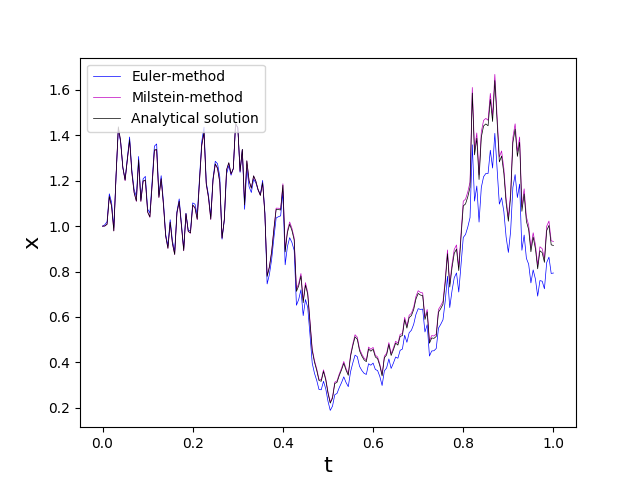
\includegraphics[width=0.6\linewidth]{Content/Graphics/slides/ApproximateSolution}
\end{figure}
\end{frame}







\section{Stochastic Integration} 
\begin{frame}
\frametitle{Terminology}
Given a probability space \(\left( \Omega , \mathcal{F}, P\right)\) and T\(\in\mathbb{R}\) finite.
\begin{definition}[Stochastic process]
Collection of random variables indexed by time:
\[X(t,\omega)\!: [0,T]\times\Omega \rightarrow \mathbb{R}\]
\end{definition}
We will use the notation: \(\{X_t\}_{t\in[0,T]}\).\\
\(X_t\) is a random variable for t\(\in[0,T]\) fixed.
\end{frame}

\begin{frame}
%Measurability\\
For each \(\omega_0\in\Omega\) fixed we can define the mapping:
\[t\mapsto X(t,\omega_0)\]
We will call this mapping a realization/\textbf{sample path}/trajectory of the stochastic process \(\{X_t\}_{t\in[0,T]}\).
\begin{figure}
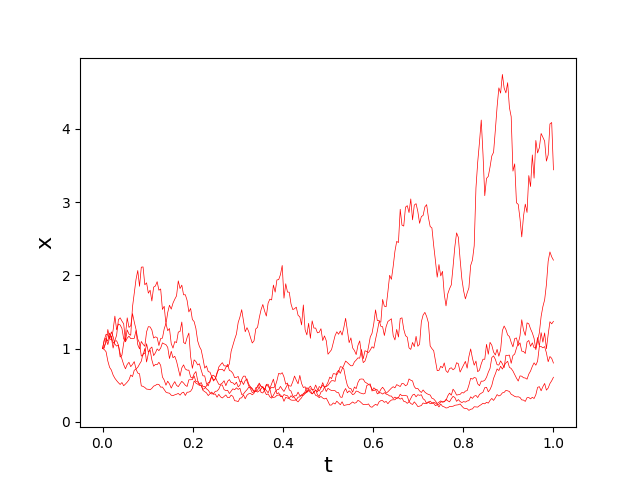
\includegraphics[width=0.6\linewidth]{Content/Graphics/slides/ExampleSamplePaths}
\end{figure}
\end{frame}


\begin{frame}
\frametitle{Terminology}
\begin{definition}[Wiener process]
The Wiener process \(\{W_t\}_{t\in[0,T]}\) is a stochastic process with the following properties:
\begin{enumerate}
\item \(W_0 = 0\)
\item \(W_t - W_s\sim\mathcal{N}(0,t-s)\)
\item \(W_{t_{1}} - W_{s_{1}}, W_{t_{2}}-W_{s{2}}\) are independent for disjoint intervals \([s_1,t_1],\,\,[s_2,t_2]\).
\end{enumerate}
\end{definition}
\end{frame}


\begin{frame}
\frametitle{Terminology}
Possible sample paths of the \textbf{discretized} Wiener process.\\
\begin{figure}
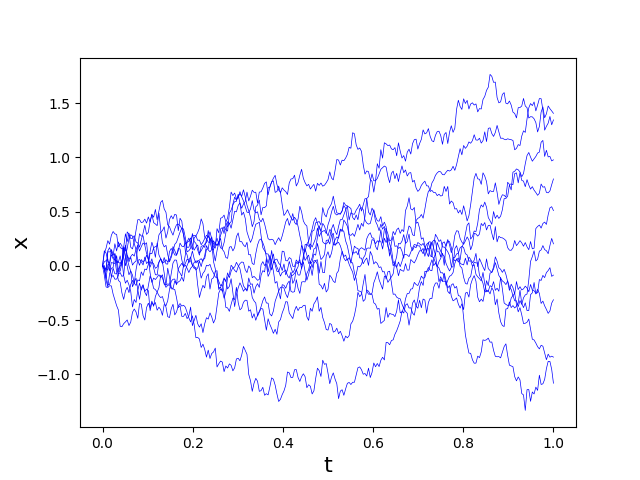
\includegraphics[width=0.75\linewidth]{Content/Graphics/slides/SamplingWiener}
\end{figure}
\end{frame}


\begin{frame}
\frametitle{The first stochastic integral}
We want to define:
\[\int_0^T \! 2W_t \, \mathrm{d}W_t.\]

reasonable approximations:\\
Given \(P_n\) partition of [0,T] with n equidistant time steps.
\[R_1(P_n) \coloneqq \sum_{k=0}^{n-1}2W_{t_k}\cdot(W_{t_{k+1}}-W_{t_k})\]			  
\[R_2(P_n) \coloneqq \sum_{k=0}^{n-1}2W_{t_{k+1}}\cdot(W_{t_{k+1}}-W_{t_k})\]
\end{frame}


\begin{frame}
\frametitle{The first stochastic integral}
We want to define:
\[\int_0^T \! 2W_t \, \mathrm{d}W_t.\]

It is possible to show:
\begin{lemma}
\[R_1(P_n) \rightarrow W_T^2 - T \quad  (\text{in } L^2[\Omega])\text{ as }n\to\infty\]
\[R_2(P_n) 	\rightarrow W_T^2 + T \quad       (\text{in } L^2[\Omega])\text{ as }n\to\infty\]
\end{lemma}
\end{frame}


\begin{frame}

\textbf{Questions:}
\begin{enumerate}
\item Which definition to use? (It\^o)
\item For which stochastic processes \(\{X_t\}_{t\in[0,T]}\) is it possible to define the  It\^o stochastic integral:
\[\int_0^T \! X_t \, \mathrm{d}W_{t}\,?\]
\end{enumerate}


\end{frame}



\begin{frame}
\frametitle{Terminology}
\begin{definition}[Filtration induced by the Wiener process]
Filtration \(\mathcal{F^W}_t\coloneqq\sigma(\{W_s\mid 0\leq s\leq t\})\) for t\;\(\in[0,T]\).\\
\(\{\mathcal{F^W}_t\}_{t\in[0,T]}\) is an increasing sequence of \(\sigma\)-algebras.
\end{definition}
\begin{definition}[Adapted process]
We will call \(\{X_t\}_{t\in[0,T]}\) to be \(\mathcal{F^W}_t\)-adapted if it is \(\mathcal{F^W}_t\)-measurable \(\forall\; t\in[0,T].\)
\end{definition}

\end{frame}




\begin{frame}
\frametitle{Terminology}
\begin{definition}[\(L^2\)-norm for stochastic processes]
\(\|\{X_t\}_{t\in[0,T]}\|_{L^2[0,T]}\coloneqq\mathbb{E}[\int^{T}_{0}X_t^2\mathrm{d}t]^\frac{1}{2}\)
\end{definition}


\begin{definition}[Class of adapted, square-integrable processes]
\[C \coloneqq \{X\!: [0,T]\times\Omega \rightarrow \mathbb{R}\mid  Properties \}.\]
\end{definition}

\textbf{Properties}
\begin{enumerate}
\item \(\{X_t\}_{t\in[0,T]} \text{ is measurable}\)     
\item \(\|\{X_t\}_{t\in[0,T]}\|_{L^2[0,T]}<\infty\)
\item \(\{X_t\}_{t\in[0,T]}\) is \(\mathcal{F^W}_t\)-adapted 
\end{enumerate}
\end{frame}

%\begin{frame}
%\frametitle{Terminology}
%\begin{definition}[Class of random step functions]
%\(\mathcal{E}\) is the class of stochastic processes which can be written in the following form:
%\[\xi_t^{n} = \sum^{n-1}_{k=0}Z_k\cdot\mathbbm{1}_{[t_k,t_{k+1})}\]
%for a partition of [0,T] and some random variables \(Z_k \:\:\mathcal{F}_{t_k}\)-measurable and square-integrable for \(k=0,\cdots,n-1.\)
%\end{definition}
%Sample paths of such functions are step functions. 
%
%\begin{lemma}
%\(\mathcal{E}\) is dense in \(\mathcal{C}\).
%\end{lemma}
%\end{frame}

%\begin{frame}
%\frametitle{Stochastic-Integration}
%
%\begin{definition}[Stochastic integral for step functions]
%\[\int_0^T \! \xi_t^{n}\, \mathrm{d}W_{t}\coloneqq\sum^{n-1}_{k=0}Z_k\cdot(W_{t_{k+1}}-W_{t_{k}})\]
%\end{definition}
%
%\end{frame}



\begin{frame}
\frametitle{Stochastic integration}
For each \(\{X_t\}_{t\in[0,T]}\) \(\in\mathcal{C}\) the It\^o stochastic integral 
\[\int_0^T\! X_t\,\mathrm{d}W_{t}\]
exists as an element in \(L^2[\Omega]\).\\

\textbf{Construction:}\\
Via "random step functions"

%It is defined as the limit in \(L^2[\Omega]\) of stochastic integrals of random step functions:

%\[\lim_{n\to\infty}\int_0^T\! \xi_t^n\,\mathrm{d}W_{t}\quad\quad (\xi_t^n)_{n\!\in\!\mathbb{N}}\in\mathcal{E}\]
%such that
% \(\|X_t-\xi_{t}^n\|^2_{L^2[0,T]}\rightarrow 0\:\text{as}\:n\rightarrow\infty\)
%%%%%%(\mathbb{E}[\int_{0}^{T}(X_t-\xi_{t}^n)^2\mathrm{d}t] = 
\end{frame}


\begin{frame}
\frametitle{Stochastic integration}
\begin{theorem}[It\^o isometry]
Let \(X_t\!\in\mathcal{C}\). Then
\[\mathbb{E}[(\int_0^T\!X_t\,\mathrm{d}W_{t})^2] = \mathbb{E}[\int_0^T\!(X_t)^2\,\mathrm{d}t]\]
\[\|\int_0^T\!X_t\,\mathrm{d}W_{t}\|_{L^2[\Omega]} = \|\{X_t\}_{t\in[0,T]}\|_{L^2[0,T]}\]
\end{theorem}
Holds only for stochastic integrals in the It\^o-sense.
\end{frame}




\begin{frame}
\frametitle{Lemma of It\^o}
Given a stochastic differential equation (Also called \textbf{It\^o-process}):
\[X_t = x_0 + \int_0^t \!a(X_s)\,\mathrm{d}s + \int_0^t \!b(X_s)\,\mathrm{d}W_{s},\quad t\in [0,T]\]
\[X_0 = x_0\,\,\text{initial value}\]

Given \textbf{a smooth map u}:\(\mathbb{R}\to\mathbb{R}\).\\

\textbf{Question:}
\begin{enumerate}
\item What is the \textbf{representation} of \(u(X_t)\)?
\end{enumerate}

\end{frame}


\begin{frame}
\frametitle{Lemma of It\^o}
Given a stochastic differential equation as before.
Given a smooth map u:\(\mathbb{R}\to\mathbb{R}\).\\

Then:
\[u(X_t)  = u(x_0) + \int_0^t \!u_x(X_s)a(X_s) + \frac{1}{2}u_{xx}(X_s)b(X_s)^2\,\mathrm{d}s +\]
\[ \int_0^t \!u_x(X_s)b(X_s)\,\mathrm{d}W_{s}\]

If we are lucky: the lemma gives us the solution of the SDE.
\end{frame}




\section{Stochastic Differential Equations} 

\begin{frame}
\frametitle{Stochastic Differential Equations}
Consider again a stochastic differential equation:
\[X_t = x_0 + \int_0^t \!a(X_s)\,\mathrm{d}s + \int_0^t \!b(X_s)\,\mathrm{d}W_{s},\quad t\in [0,T],\]
\[X_0 = x_0\,\,\text{initial value}\]

Conditions on the coefficients such that the solution \(\{X_t\}_{t\in[0,T]}\) exists and is unique.\\
We are interested in the stochastic process which solves the above equation.\\
\textbf{Examples?}
\end{frame}

\begin{frame}
\frametitle{Geometric Brownian motion}
Set \(a(x) = \mu x\) and \(b(x) = \sigma x\). Then the SDE reads:
\[X_t = x_0 + \int_0^t \!\mu X_s\,\mathrm{d}s + \int_0^t \!\sigma X_s\,\mathrm{d}W_{s}\]
Using the It\^o-lemma we can get the solution for all \(t\in[0,T]\):

\[X_t = x_0\exp({(\mu-\frac{\sigma^2}{2})t + \sigma W_t}).\]
This is the \textbf{geometric Brownian motion.}

\end{frame}


\begin{frame}
\frametitle{Ornstein-Uhlenbeck process}
Set \(a(x) = -\beta x\) and \(b(x) = \sigma\). Then the SDE reads:
\[ X_t = x_0 + \int_0^t \!-\beta X_s\,\mathrm{d}s + \int_0^t \!\sigma\,\mathrm{d}W_{s}\]
Using the It\^o-lemma we can get the solution for all \(t\in[0,T]\):

\[X_t = x_0\exp({-\beta t}) + \sigma\int_0^t \!\exp({-\beta(t-s)})\,\mathrm{d}W_{s}.\]
This is the \textbf{Ornstein-Uhlenbeck process.}

\end{frame}



\section{Numerical Analysis} 

\begin{frame}
\frametitle{Stochastic Taylor expansions}
Given a stochastic differential equation as before:
\[X_t = x_0 + \int_0^t \!a(X_s)\,\mathrm{d}s + \int_0^t \!b(X_s)\,\mathrm{d}W_{s},\quad t\in [0,T]\]
\[X_0 = x_0\,\,\text{initial value}\]

\textbf{Question:}
\begin{enumerate}
\item What happens if we apply the It\^o-lemma on \(a(x)\) and \(b(x)\) ? 
\end{enumerate}
\end{frame}

\begingroup
\small
\begin{frame}
\frametitle{Stochastic Taylor expansions}
\[a(X_s) = a(X_0) + \int_0^s \!a_x(X_r)a(X_r) + \frac{1}{2}a_{xx}(X_r)b(X_r)^2\,\mathrm{d}r + \int_0^s \!a_x(X_r)b(X_r)\,\mathrm{d}W_{r}\]
\[b(X_s) = b(X_0) + \int_0^s \!b_x(X_r)a(X_r) + \frac{1}{2}b_{xx}(X_r)b(X_r)^2\,\mathrm{d}r + \int_0^s \!b_x(X_r)b(X_r)\,\mathrm{d}W_{r}\]
\end{frame}
\endgroup

\begin{frame}
\frametitle{Stochastic Taylor expansions}
Plugging into the original equation yields:
\[X_t = x_0 + \int_0^t \!a(X_0)\,\mathrm{d}s + \int_0^t \!b(X_0)\,\mathrm{d}W_{s} + R\]
\[X_t = x_0 + a(X_0)\cdot t + b(X_0)\cdot W_{t} + R\]
\[t\in [0,T]\]

R is the remainder term.\\
This is the \textbf{1. Stochastic Taylor expansion}.
\end{frame}


\begin{frame}
\frametitle{Stochastic Taylor expansions}
A third application of the It\^o-lemma yields:
%\[X_t = x_0 + \int_0^t \!a(X_0)\,\mathrm{d}s +  \int_0^t \!b(X_0)\,\mathrm{d}W_{s} + \int_0^t \!\int_0^s \!\,b_x(X_0)b(X_0)\mathrm{d}W_{r}\,\mathrm{d}W_{s} + R\]
\[X_t = x_0 + a(X_0)t + b(X_0)W_t +  \underbrace{\frac{1}{2}b_x(X_0)b(X_0)(W_t^2-t)}_{\text{Additional term}} +  R\]
\[t\in [0,T]\]

R is the remainder term.\\
This is the \textbf{2. Stochastic Taylor expansion}.
\end{frame}

\begin{frame}
\frametitle{Stochastic Taylor expansions}
\textbf{Numerical methods for SDE's:}\\ 
Expand the equation iteratively using the It\^o-lemma and remove terms of higher order (in \(L^2[\Omega]\)-norm).\\

It is possible to show that these truncated stochastic Taylor expansions converge to \(X_t\) in \(L^2[\Omega]\).

\end{frame}

\begin{frame}
\frametitle{Euler-Method for SDE's}
\textbf{Euler-Method} for SDE's: 1. Stochastic Taylor expansion for n points \(t_1,\cdots,t_n\in[0,T]\) and remove the remainder term.\\
Defined recursively:\\
\begin{enumerate}
\item Initialize \(\overline{X}^n_{t_0}=x_0\)
\item For k = 0 to n-1
\begin{enumerate}
\item \(\overline{X}^n_{t_{k+1}} = \overline{X}^n_{t_k} + a(\overline{X}^n_{t_k})(t_{k+1}-t_k) + b(\overline{X}^n_{t_k})(W_{t_{k+1}}-W_{t_k})\)
\end{enumerate}
\item Linear interpolation.
\end{enumerate}
\end{frame}


\begin{frame}
\frametitle{Milstein-Method for SDE's}
\textbf{Milstein-Method} for SDE's: 2. Stochastic Taylor expansion for n points \(t_1,\cdots,t_n\in[0,T]\) and remove the remainder term.\\
Defined recursively:\\
\begin{enumerate}
\item Initialize \(\overline{X}^n_{t_0}=x_0\)
\item For k = 0 to n-1
\begin{enumerate}
\item \(\overline{X}^n_{t_{k+1}} = \overline{X}^n_{t_k} + a(\overline{X}^n_{t_k})(t_{k+1}-t_k) + b(\overline{X}^n_{t_k})(W_{t_{k+1}}-W_{t_k})
+ \frac{1}{2}b(\overline{X}^n_{t_k})b_x(\overline{X}^n_{t_k})((W_{t_{k+1}}-W_{t_k})^2-(t_{k+1}-t_k))\)
\end{enumerate}
\item Linear interpolation.
\end{enumerate}
\end{frame}


\begin{frame}
\frametitle{Illustration}
Approximation of the sample paths of the geometric Brownian motion.\\
Using the \textbf{Euler} and the \textbf{Milstein} method.
\begin{figure}[!h]
\centering
   \begin{subfigure}{0.49\linewidth} \centering
     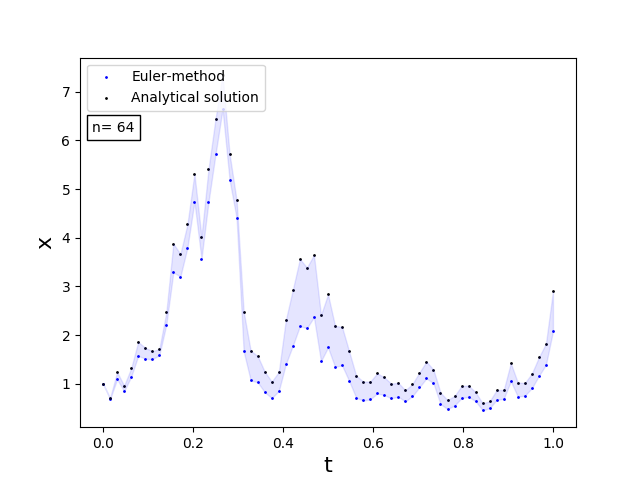
\includegraphics[scale=0.35]{Content/Graphics/SDE_EulerGBM_n_64}
   \end{subfigure}
   \begin{subfigure}{0.49\linewidth} \centering
     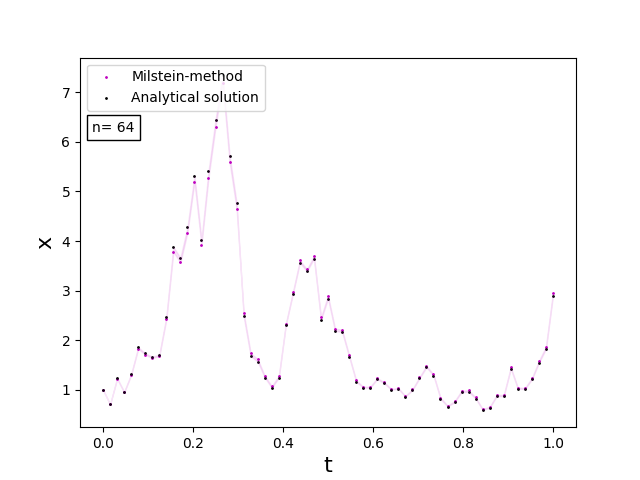
\includegraphics[scale=0.35]{Content/Graphics/SDE_MilsteinGBM_n_64}
   \end{subfigure}
\end{figure}

\end{frame}



\begin{frame}
\frametitle{Numerical analysis}
How to measure the \textbf{approximation error}?\\
\(\{\overline{X}^n_{t}\}_{t\in[0,T]}\) is the approximation for n points, linearly interpolated.\\
\(\{X_{t}\}_{t\in[0,T]}\) is the true, analytical solution.\\
\begin{block}{Approximation error}
possible criterion for the approximation error:\\
\(e_n\coloneqq\mathbb{E}[(X_T - \overline{X}^n_{T})^2]^{\frac{1}{2}}\quad\)
\end{block}
\end{frame}

\begin{frame}
\frametitle{Numerical analysis}
How to measure the \textbf{convergence order} of the methods?\\
\begin{block}{Convergence order - Error bound}
\[e_n \leq K\cdot n^{-\gamma}\]
For some constants.\\
\(\gamma\) is called the \emph{strong order of convergence} of the method.
\end{block}

How to estimate \(\gamma\)?\\
- Analytically\\
- Simulation\\

\end{frame}


\begin{frame}
\frametitle{Numerical analysis}

It is possible to show:\\
- Euler-Method has order of convergence 0.5\\
- Milstein-Method has order of convergence 1.0\\

\end{frame}



\begin{frame}
\Huge{\centerline{The End}}
\end{frame}



\end{document} 





